% !TEX root = ../../../main.tex
% 来源：高中物理甲种本·第二册（热学·电学）
% 章节：固体和液体的性质 / 液体的表面现象
% 原始文件：4.tex，行 214-227
% 类型：tikz
% ---
	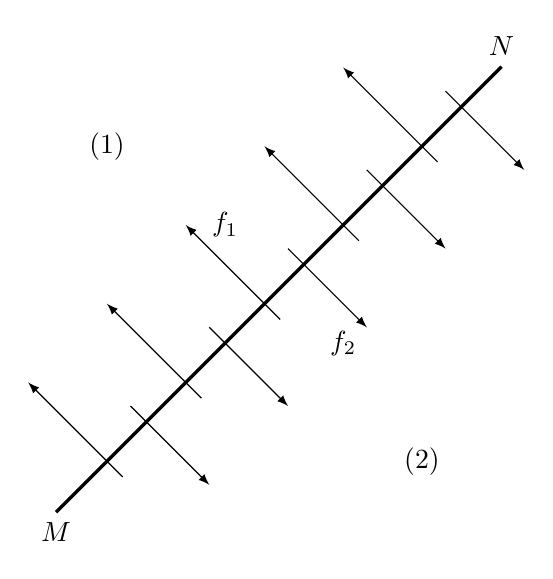
\begin{tikzpicture}[>=latex, scale=1 ]

\draw [very thick](45:.5)node[below]{$M$}--(45:8.5)node[above]{$N$};

\foreach \x in {1,2,...,5}
{ 
   \draw[->] (\x+.2,\x-.2)--(\x-1,\x+1);
   \draw[->] (\x+.5-.2,\x+.5+.2)--(\x+1.5-.2,\x-.5+.2);
}

\node at (1,5){(1)}; \node at (5,1){(2)};
\node at (4,2.5){$f_2$}; \node at (2.5,4){$f_1$};

\end{tikzpicture}
